\documentclass[12pt,a4paper]{article}

\usepackage[T1]{fontenc}
\usepackage[charter]{mathdesign}
\usepackage{amsmath,amsthm,enumitem,graphicx,titlesec,xcolor}
\usepackage{microtype}
\usepackage[a4paper,margin=25mm]{geometry}
\usepackage[unicode]{hyperref}

\hypersetup{
    hidelinks,
    pdftitle={Distributed Algorithms},
    pdfauthor={Juho Hirvonen and Jukka Suomela},
}

\definecolor{titlecolor}{HTML}{0088cc}
\definecolor{hlcolor}{HTML}{f26924}

\newcommand{\q}[2]{\paragraph{\mbox{Question #1: }#2.}}
\newcommand{\sep}{{\centering \raisebox{-3mm}[0mm][0mm]{$*\quad*\quad*$}\par}}
\newcommand{\hl}[1]{\textbf{\emph{#1}}}
\newcommand{\cemph}[1]{\textcolor{hlcolor}{\emph{#1}}}
\DeclareMathOperator{\re}{re}

\setitemize{noitemsep,leftmargin=3ex}

\titleformat{\paragraph}[runin] {\normalfont\normalsize\bfseries\color{titlecolor}}{\theparagraph}{1em}{}

\begin{document}

\noindent
\emph{CS-E4510 Distributed Algorithms / Juho Hirvonen, Jukka Suomela\\
second exam, 10 December 2020}

\paragraph{Instructions.}

There are five questions, and you must answer \hl{at least four questions} in order to pass the exam.

You are free to look at any source material (this includes lecture notes, textbooks, and anything you can find with Google), but you are not allowed to collaborate with anyone else or ask for anyone's help (this includes collaboration with other students and asking for help in online forums).

You are free to use any results from the lecture notes directly (including the results from the regular exercises). You are free to use computers and computer programs to find solutions.

If you cannot solve a problem entirely, please try to at least explain what you tried and what went wrong.

\sep

\q{1}{Maximal matching}

Consider the following graph $G_1$ with 16 nodes:
\begin{center}
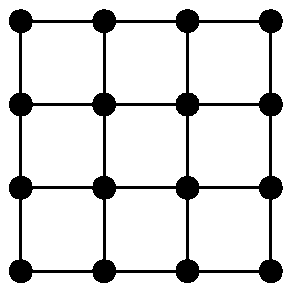
\includegraphics[page=1,scale=0.5]{figs.pdf}
\end{center}
Design a deterministic PN-algorithm $A$ that finds a \hl{maximal matching} in graph $G_1$. That is, if you run $A$ in any simple port-numbered network $N$ that has graph $G_1$ as the underlying graph, algorithm $A$ will stop and output a maximal matching.

The local inputs of the nodes are empty. Any running time is fine. A brief, informal description of the algorithm is sufficient. The algorithm does not need to do anything meaningful if you run it in any other graph.

\q{2}{Edge coloring}

Let graph $G_1$ be as defined in question~1. Prove that there is no deterministic PN-algorithm that solves the following problem: finding a \hl{proper edge coloring} (with any number of colors) in graph $G_1$.

\bigskip\noindent
\emph{Hint:} You are expected to use an argument based on covering maps.

\vspace{\stretch{1}}
\noindent\emph{There is more, please see the other page\ldots}

\newpage

\q{3}{Two colors}

Design a deterministic PN-algorithm that solves the following problem in $O(1)$ rounds:
\begin{itemize}
    \item Graph family: bipartite graphs.
    \item Local inputs: proper vertex coloring with $2$ colors.
    \item Local outputs: label the edges with labels R, G, and B such that for any node $v$ of degree at least $10$, the edges incident to $v$ use \hl{at least two different labels}.
\end{itemize}
A brief, informal description of the algorithm is sufficient.

\q{4}{Three colors}

Prove that there is no deterministic PN-algorithm that solves the following problem in $O(1)$ rounds:
\begin{itemize}
    \item Graph family: bipartite graphs.
    \item Local inputs: proper vertex coloring with $2$ colors.
    \item Local outputs: label the edges with labels R, G, and B such that for any node $v$ of degree at least $10$, the edges incident to $v$ use \hl{all three labels}.
\end{itemize}
\emph{Hints:} Consider $(10,10)$-biregular trees. Compare with the sinkless orientation problem.

\q{5}{One red, one green}

Consider the following problem in $(10,10)$-biregular trees: label the edges with labels R, G, and B such that for any node $v$ of degree $10$, the edges incident to $v$ use label R \hl{exactly once} and label G \hl{exactly once}.
\begin{enumerate}[label=(\alph*)]
\item Formalize this as a \emph{bipartite locally verifiable problem} $\Pi$ (Section 9.1.1 in the lecture notes).
\item Show that $\Pi$ is not solvable in $0$ rounds.
\item Show that $\Pi$ is a periodic point in round elimination, i.e., if you apply $\re$ sufficiently many times, you will arrive at a problem equivalent to $\Pi$.
\item How long is the period, i.e., how many applications of $\re$ are needed to arrive at the original problem $\Pi$?
\end{enumerate}

\end{document}
